
\begin{frame}{Heurística ASV: Recordando la Fórmula}
	\small
	\dificultyLevel{2}
	Recordemos la definición de ASV:
	\[
	    \assym_{M,e,\Pr}(x_i)
	    \;=\;
	    \frac{1}{|\topo(G)|}\sum_{\pi \in \topo(G)} 
	      \Bigl(\charactheristicFunction(\pi_{<i} \cup \{x_i\})
	      \;-\;\charactheristicFunction(\pi_{<i})\Bigr).
	\]
	\begin{itemize}[<+- | alert@+>]
	    \item Nuestro objetivo es minimizar la cantidad de veces que se evalúa $\charactheristicFunction$.
	    \item La idea de la heurística es identificar los órdenes topológicos que devuelven el mismo resultado al ser evaluados por $\charactheristicFunction$. 
	    \item Así solo tendremos que evaluar $\charactheristicFunction$ una vez por cada orden perteneciente a cada clase de equivalencia. 
	\end{itemize}
	% \only<4>{\begin{mydefinition}[Clase de equivalencia $\rel$] 	Sea \(A\) un conjunto y \(R \subseteq A \times A\) una relación de equivalencia. La clase de equivalencia $[a]_\rel$ son todos los elementos de $A$ relacionados con $a$.
	%Para cada \(a \in A\), la \emph{clase de equivalencia} de \(a\) bajo \(R\) se define como
	%\[	[a]_R \;=\; \{\,x \in A \mid a \ R \ x \}.	\] 	\end{mydefinition}}
	\only<2>{ 
		\alert{Podemos agruparlos según la relación $\rel^\star$, en la cual dos órdenes topológicos \(\pi^1,\pi^2\) están relacionados si evaluán a lo mismo.} %($\charactheristicFunction(\pi^1_{<i}) \;=\; \charactheristicFunction(\pi^2_{<i})$).
		}
\end{frame}

\begin{comment}
	\begin{frame}{Introducción a $\rel$}
		\dificultyLevel{2}
		\begin{itemize}[<+- | alert@+>]
			\item En la siguiente sección vamos a introducir la relación $\rel$, se define sobre los órdenes topológicos de nuestro grafo causal $G$. 
			\item Luego, para calcular las distintas clases de equivalencia vamos a tener que establecer ciertas relaciones entre los nodos y los órdenes de $G$. 
			\item Más adelante vamos a ver cómo contar los órdenes topológicos, ya que nos va a ayudar a calcular los tamaños de estas clases. 
			\item Por último, vamos a encontrar una cota para el número de clases de equivalencia de un \dtree. 
		\end{itemize}
	\end{frame}
\end{comment}


% ---------------------------------------------------------
\begin{frame}{Relación de Equivalencia \(\rel\)}
\dificultyLevel{3}
%\only<1>{Como \(\rel^\star\) es díficil de calcular, definimos una relación \(\rel\) más manejable.}
Definimos \(\rel\) para distinguir clases de equivalencia \(\equivalenceClass\)
para el feature \(x_i\):
\[
  \pi^1 \rel \; \pi^2 
  \quad\Longleftrightarrow\quad
  \{\pi^1_{<i}\} \;=\; \{\pi^2_{<i}\}
\]
\only<1>{%es decir, dos órdenes topológicos están en la misma clase si,  previo a la posición de \(x_i\), tienen el mismo conjunto de nodos.
	Ambos órdenes evaluan igual: $\alert{\charactheristicFunction(\pi_{<i})}$. }


\only<2>{
	\begin{figure}
		\centering
		\includegraphics[width=0.8\linewidth]{pic/img/SHAP/equivalenceClassTopoSortNotEqual.png}
	\end{figure}
}

\only<3>{
	\begin{figure}
		\centering
		\includegraphics[width=0.8\linewidth]{pic/img/SHAP/equivalenceClassTopoSortEqual.png}
	\end{figure}
}

\end{frame}

\begin{frame}{Heuristíca ASV}
	\dificultyLevel{2}
	Denotemos por 
	\[
	eqCl(G,x_i) \;=\; \{\,[\pi]_{\rel} \mid \pi \in \topo(G)\}
	\]
	al conjunto de clases de equivalencia respecto de \(\rel\). \pause Entonces nuestra fórmula original nos queda:
	\[
	%\assym_{M,e,\Pr}(x_i)
	%\;=\; 
	\frac{1}{|\topo(G)|}\sum_{\alert{[\pi]_{\rel} \,\in\, eqCl(G,x_i)}} 
	\Bigl(\charactheristicFunction(\pi_{<i} \cup \{x_i\}) 
	- \charactheristicFunction(\pi_{<i})\Bigr) 
	\;\cdot\; \alert{\bigl|\,[\pi]_{\rel}\bigr|}
	\]    
	en vez de: 
	\[
	%\assym_{M,e,\Pr}(x_i)
	%\;=\;
	\frac{1}{|\topo(G)|}\sum_{\pi \in \topo(G)} 
	\Bigl(\charactheristicFunction(\pi_{<i} \cup \{x_i\})
	\;-\;\charactheristicFunction(\pi_{<i})\Bigr)
	\]
\end{frame}


\begin{comment}
	\begin{mydefinition}[Clase de equivalencia de \(\rel\)]
		Sea \(D=(V,E)\) y \(x_i\in V\). Para \(\pi\in \topo(G)\), definimos 
		$f_{\pi}$ tal que $f_{\toOr}(n)$ es una función que identifica si el nodo $n$ está a la derecha o izquierda de $x_i$ en $\toOr$. \pause
		\begin{itemize}[<+- | alert@+>]
			\item La clase de equivalencia \(\equivalenceClass\) se representa con $\equivalenceClassRep$ por $V$ etiquetado por $f_{\pi}$. 
			%\(   \equivalenceClassRep     = \{\,v_{f_{\pi}(v)} \mid v \in V\setminus\{x_i\}\}.  \) 
			%\item $L(\equivalenceClass)$ y $R(\equivalenceClass)$ denotan el conjunto de nodos a la izquierda y a la derecha en la clase de equivalencia, respectivamente.
		\end{itemize}
	\end{mydefinition}
	
	\begin{frame}{Relación de Equivalencia $\rel$}
		\dificultyLevel{3}
		\begin{mydefinition}[Pertenencia a una clase]\label{def:belongsEquivClass}
			Sea $G$ un digrafo $G = (V, E)$. Un orden topológico $\toOr'$ pertenece a la clase de equivalencia $\equivalenceClass$ si se cumple que tiene los mismos nodos a la izquierda de $x_i$ que $\toOr$.
			\small
			%$$  (\forall v \in V \setminus \{x_i\}) (f_{\toOr'}(v) = left \land v \in L(\equivalenceClass) ) \lor (f_{\toOr'}(v) = right \land v \in R(\equivalenceClass) )    $$
			
		\end{mydefinition}
		
	\end{frame}
	\pause
	\smallskip
	\emph{Observación:} \(\rel\) es más fina que \(\rel^\star\). 
	Si dos órdenes tienen el mismo conjunto antes de \(x_i\), 
	no necesitamos evaluar \(\charactheristicFunction\) para agruparlos.
	
	% ---------------------------------------------------------
	%Si esto hubiera sobrevivido hubiera habido que se hacer más enfasis en que esto se utiliza para calcular los tamaños de las clases
	\begin{frame}{Número de Órdenes Topológicos en un DAG}
		\dificultyLevel{2}
		\small
		Queremos una fórmula para \(\lvert \topo(G)\rvert\) en familias especiales de DAGs, 
		porque en general es \(\sharpPhard\) \cite{countingLinearExtensions}. \only<1>{Esto lo vamos a necesitar para calcular los tamaños de las clases de equivalencia.} \pause 
		
		\medskip
		\textbf{Caso base: grafo vacío con \(r+1\) nodos (sin aristas).}
		\[
		\lvert \topo(G)\rvert = (r+1)!.
		\]
		\begin{figure}
			\centering
			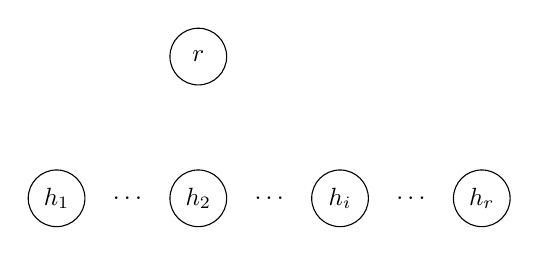
\begin{tikzpicture}[scale=0.9, transform shape,
				nodo/.style={circle, draw, minimum size=0.8cm}]
				\node[nodo] (r)   at (0, 0) {$r$};
				\node[nodo] (h1)  at (-2,-2) {$h_1$};
				\node[nodo] (h2)  at (-0,-2) {$h_2$};
				\node[nodo] (hi)  at (2,-2) {$h_i$};
				\node[nodo] (hr) at (4,-2) {$h_r$};
				\node[draw=none, fill=none]  (dotsL) at (-1,-2) {$\ldots$};
				\node[draw=none, fill=none]  (dotsR) at (1,-2) {$\ldots$};
				\node[draw=none, fill=none]  (dotsRR) at (3,-2) {$\ldots$};
			\end{tikzpicture}
			\caption*{DAG sin aristas: todos los nodos son permutables.}
			\label{fig:emptyGraphExample}
		\end{figure}
	\end{frame}
	
	% ---------------------------------------------------------
	\begin{frame}{Conteo de Órdenes en \dtrees}
		\dificultyLevel{2}
		
		\small
		Ahora añadimos aristas para formar un \dtree. Sea \(D\) un \dtree\ con raíz \(r\). 
		
		
		
		\begin{figure}[ht]
			\centering 
			\begin{tikzpicture}[scale=.6, transform shape]
				
				% ---- NODOS ----
				\node[nodo] (r) at (0, 0) {$r$};
				\node[nodo] (s1) at (-4, -2) {$h_1$};
				\node[nodo] (s2) at (-2, -2) {$h_2$};
				\node[nodo] (si) at (1, -2) {$h_i$};
				\node[nodo] (sn-1) at (4, -2) {$h_{r}$};
				
				\node[draw=none, fill=none] (dots) at (-0.2, -2) {$\ldots$}; % Ellipsis
				\node[draw=none, fill=none] (dots) at (2.2, -2) {$\ldots$}; % Ellipsis
				
				\node[draw=none, fill=none] (h1) at (-4, -4) {};
				\node[draw=none, fill=none] (h2) at (-2, -4) {};
				\node[draw=none, fill=none] (hi) at (1, -4) {};
				\node[draw=none, fill=none] (hn-1) at (4, -4) {};
				
				
				\path [->] (r) edge[arista]  (s1);
				\path [->] (r) edge[arista]  (s2);
				\path [->] (r) edge[arista]  (si);
				\path [->] (r) edge[arista]  (sn-1);
				
				\path [->] (s1) edge[arista,  mySnake]  (h1);
				\path [->] (s2) edge[arista,  mySnake]  (h2);
				\path [->] (si) edge[arista,  mySnake]  (hi);
				\path [->] (sn-1) edge[arista,  mySnake]  (hn-1);
			\end{tikzpicture}
			\caption*{Polytree con nodos con grados de entrada menores o iguales a 1, lo cual definimos como \dtree.}
			\label{fig:dtreeExample}
		\end{figure}
	\end{frame}
	
	\begin{frame}{Conteo de Órdenes en \dtrees}
		\dificultyLevel{3}
		\textbf{Fórmula general:}
		
		\only<1>{
			\begin{mydefinition}
				Sean \(k_i\) la cantidad de nodos del subárbol \(t_i\), con 
				\(n = \sum_{i=1}^r k_i\). La cantidad de órdenes topológicos es:
			\end{mydefinition}
		}
		
		\only<2>{
			\begin{mydefinition}
				Sean \(k_i\) la cantidad de nodos del subárbol \(t_i\), con 
				\(n = \sum_{i=1}^r k_i\). La cantidad de órdenes topológicos es:
				\[
				\numTopo(t) 
				= \alert<2>{\binom{n}{k_1,\dots,k_r}}
				\]
			\end{mydefinition}
		}
		
		\only<3->{
			\begin{mydefinition}[Órdenes Topológicos en un \dtree]
				Sean \(k_i\) la cantidad de nodos del subárbol \(t_i\), con 
				\(n = \sum_{i=1}^r k_i\). La cantidad de órdenes topológicos es:
				\[
				\numTopo(t) 
				= \binom{n}{k_1,\dots,k_r}
				\;\cdot\;
				\alert<3>{\prod_{i=1}^{r} \numTopo(t_i)}
				\]
			\end{mydefinition}
		}
		
		\begin{itemize}
			\item<2-> \alert<2>{Coeficiente multinomial: 
				\(\binom{n}{k_1,\dots,k_r} = \frac{n!}{k_1!\cdots k_r!}\)} 
			cuenta las maneras de intercalar nodos de subárboles sin alterar su orden interno.
			\item<3-> \alert<3>{Producto de subárboles: 
				\(\prod_{i=1}^{r} \numTopo(t_i)\)} 
			corresponde a las combinaciones posibles dentro de cada subárbol.
			\item<4-> \alert<4>{Combinación final: la fórmula multiplica ambas partes para obtener el total de órdenes topológicos.}
		\end{itemize}
	\end{frame}
	
	\begin{frame}{Extensión a \textit{Polyforests} con Raíz Virtual}
		\dificultyLevel{2}
		\small
		Si nuestro DAG es un \emph{polyforest} (varias raíces \(r_1,\dots,r_\ell\)), 
		podemos agregar una raíz virtual \(r_0\) que conecte a todas las raíces originales. 
		\(r_0\) actúa como raíz de un \dtree\ que engloba todo el polyforest:
		
		\begin{figure}[ht]
			\centering 
			\begin{tikzpicture}[scale=.6, transform shape]
				
				% ---- NODOS ----
				\node[nodo, blue] (r) at (0, 0) {$r_0$};
				\node[nodo] (s1) at (-4, -2) {$r_1$};
				\node[nodo] (s2) at (-2, -2) {$r_2$};
				\node[nodo] (si) at (1, -2) {$r_i$};
				\node[nodo] (sn-1) at (4, -2) {$r_{l}$};
				
				\node[draw=none, fill=none] (dots) at (-0.2, -2) {$\ldots$}; % Ellipsis
				\node[draw=none, fill=none] (dots) at (2.2, -2) {$\ldots$}; % Ellipsis
				
				\node[draw=none, fill=none] (h1) at (-4, -4) {};
				\node[draw=none, fill=none] (h2) at (-2, -4) {};
				\node[draw=none, fill=none] (hi) at (1, -4) {};
				\node[draw=none, fill=none] (hn-1) at (4, -4) {};
				
				
				\path [->] (r) edge[arista, blue]  (s1);
				\path [->] (r) edge[arista, blue]  (s2);
				\path [->] (r) edge[arista, blue]  (si);
				\path [->] (r) edge[arista, blue]  (sn-1);
				
				\path [->] (s1) edge[arista,  decorate, decoration={snake, amplitude=.4mm, segment length=4mm, post length=1mm}]  (h1);
				\path [->] (s2) edge[arista,  decorate, decoration={snake, amplitude=.4mm, segment length=4mm, post length=1mm}]  (h2);
				\path [->] (si) edge[arista,  decorate, decoration={snake, amplitude=.4mm, segment length=4mm, post length=1mm}]  (hi);
				\path [->] (sn-1) edge[arista,  decorate, decoration={snake, amplitude=.4mm, segment length=4mm, post length=1mm}]  (hn-1);
			\end{tikzpicture}
			\caption*{El DAG original son los nodos y aristas en negro, el nodo virtual y sus aristas están en azul.}
			\label{fig:topoSortCalcForForests}
		\end{figure}
		
		Así, usamos la misma fórmula multinomial 
		\(\numTopo(t)\) vista para \dtrees, ahora aplicable a polyforests.
	\end{frame}
\end{comment}


\begin{comment}
	
	% ---------------------------------------------------------
	\begin{frame}{Más definiciones: Ancestros, Descendientes y Nodos No Relacionados}
		\dificultyLevel{2}
		\begin{figure}[ht]
			\centering 
			\begin{tikzpicture}[scale=.8, transform shape]
				
				% ---- NODOS ----
				\node[nodo] (a1) at (0, 0) {$a_1$};
				\node[nodo] (a2) at (2.5, 2) {$a_2$};
				\node[nodo] (a3) at (2.5, -2) {$a_3$};
				\node[nodo] (xi) at (5, 0) {$x_i$};
				\node[nodo] (d1) at (7.5, 2) {$d_1$};
				\node[nodo] (d2) at (10, -2) {$d_2$};
				\node[nodo] (d3) at (10, 0) {$d_3$};
				
				\node[draw=none, fill=none] (hijoa3) at (4.5, -4) {};
				\node[draw=none, fill=none] (hijod2) at (8, -4) {};
				
				% ---- ARISTAS ----
				\path [->] (a1) edge[arista, mySnake]  (xi);
				\path [->] (a2) edge[arista, mySnake]  (xi);
				\path [->] (a3) edge[arista, mySnake]  (xi);
				\path [->] (xi) edge[arista, mySnake]  (d1);
				\path [->] (xi) edge[arista, mySnake]  (d2);
				\path [->] (xi) edge[arista, mySnake]  (d3);
				\path [->] (a3) edge[arista, mySnake] node[above right] {descendientes de $a_3$ } (hijoa3);
				\path [->] (hijod2) edge[arista, mySnake] node[below right] {ancestros de $d_2$ } (d2);
				
			\end{tikzpicture}
			\caption*{Al fijar un nodo $x_i$, podemos dividir el resto de los nodos en tres grupos: \textit{ancestros} (todos los nodos que pueden alcanzar a $x_i$), \textit{descendientes} (todos los nodos alcanzables desde $x_i$) y aquellos \textit{no relacionados} con $x_i$.} %Los \textit{no relacionados} son los que no pertenecen a los ancestros ni a los descendientes, por lo que pueden estar a la derecha o la izquierda de $x_i$ en un orden topológico.}
		\label{fig:unrelatedNodesDefinition}
	\end{figure}
	\end{frame}
	
	\begin{frame}{Ancestros, Descendientes y Nodos No Relacionados}
		\dificultyLevel{2}
		\begin{itemize}[<+->]
			\item Sea \(A\) el conjunto de ancestros de \(x_i\) y \(D\) el de descendientes.
			\item Para cualquier \(\pi\in \topo(G)\), los nodos de $A$ siempre van a estar a la izquierda de $x_i$ y los nodos de $D$ a la derecha.
			\item Los \emph{nodos no relacionados} \(U = V \setminus (A\cup D\cup\{x_i\})\) 
			pueden ubicarse a la izquierda o a la derecha de \(x_i\), por lo tanto son los que definen las clases de equivalencia.
		\end{itemize}
	\end{frame}
\end{comment}

% ---------------------------------------------------------
\begin{frame}{Clases de Equivalencia en \dtrees: Ejemplo}
	\dificultyLevel{2}
	\begin{figure}[ht]
		\centering 
		\begin{tikzpicture}[scale=.5, transform shape, 
			unrelated/.style={circle, draw=red},
			wiggly/.style={decorate, decoration={snake, amplitude=.2mm, segment length=2mm}}  % Define wiggly line style
			]
			
			% ---- NODOS ----
			\node[nodo, blue] (r) at (0, 0) {$r$};
			\node[unrelated] (a1) at (-1, -2) {$a_1$};
			\node[nodo, blue] (a2) at (1, -2) {$a_2$};
			
			\node[unrelated] (b1) at (-1, -4) {$b_1$};
			\node[nodo, blue] (b2) at (1, -4) {$b_2$};
			\node[unrelated] (b3) at (3, -4) {$b_3$};
			
			\node[unrelated] (c1) at (0, -7) {$c_1$};
			\node[nodo, blue] (c2) at (3, -6) {$c_2$};
			
			% Nodo x_i ampliado
			\node[nodo, font=\Large, minimum size=1cm] (xi) at (3, -8) {$x_i$};
			
			\node[draw=none, fill=none] (hi) at (3, -10) {};
			
			\path [->] (r) edge[arista]  (a1);
			\path [->] (r) edge[arista]  (a2);
			
			\path [->] (a2) edge[arista]  (b1);
			\path [->] (a2) edge[arista]  (b2);
			\path [->] (a2) edge[arista]  (b3);
			
			\path [->] (b2) edge[arista]  (c1);
			\path [->] (b2) edge[arista]  (c2);
			
			\path [->] (c2) edge[arista]  (xi);
			
			
			\node[text=red, font=\Large] at (-2, -8) {$c_1$ subárbol}; 
			\draw[red, wiggly] (-1, -9) -- (0,-7.4) -- (1, -9) -- cycle;  % Draw the triangle
			
			\node[text=red, font=\Large] at (-3, -5) {$b_1$ subárbol}; 
			\draw[red, wiggly] (-2, -6) -- (-1,-4.4) -- (0, -6) -- cycle;  % Draw the triangle
			
			\path [->, teal] (xi) edge[arista,  decorate, decoration={snake, amplitude=.4mm, segment length=4mm, post length=1mm}] node[right, font=\Large] {descendientes de $x_i$} (hi);
		\end{tikzpicture}
		\caption*{Ejemplo de un \dtree{} con $x_i$ en negro, sus nodos no relacionados marcados en rojo y sus ancestros marcados en azul.} %Llamemos $UR$ al conjunto de raíces de los árboles no relacionados. }
		\label{fig:dtreeForestForEquivalenceClasses}
	\end{figure}
	
\end{frame}

\begin{comment}
	\begin{frame}{Clases de Equivalencia en \dtrees: Ejemplo}
		\dificultyLevel{2}
		\begin{itemize}[<+->]
			\item Solo los nodos en rojo (\(b_1,\,b_3,\,c_1,\dots\)) pueden variar 
			izquierda/derecha respecto a \(x_i\) y definir nuevas clases.
			\item Si no hubiera aristas entre subárboles rojos, habría \(2^{|U|}\) clases 
			(cada nodo de \(U\) puede ir a la izquierda o derecha). 
			\item Sin embargo, las aristas internas en cada subárbol imponen restricciones.
		\end{itemize}
	\end{frame}
\end{comment}


% ---------------------------------------------------------
\begin{frame}{Subárbol de Nodos No Relacionados: Ejemplo}
	\dificultyLevel{2}
	\small
	Tomemos el subárbol de \(b_1\) del ejemplo. 
	Queremos ver las clases de equivalencia posibles dentro de dicho subárbol:
	%\[	b_1	\;\to\; 	\bigl\{\,1_1,\;1_2\,\bigr\}	\;\to\; \bigl\{\,2_1,\;2_2,\;2_3\,\bigr\}.	\]
	\begin{figure}
		\centering
		\begin{tikzpicture}[scale=0.9, transform shape,
			unrelated/.style={circle, draw=red, thick, minimum size=0.8cm},
			arista/.style={->, thick, >=Stealth},
			wiggly/.style={decorate, decoration={snake, amplitude=.2mm, segment length=2mm}}]
			
			% ---- NODOS ----
			\node[unrelated] (b1) at (0,  0) {$b_1$};
			\node[unrelated] (11) at (-1,-2) {$1_1$};
			\node[unrelated] (12) at (1, -2) {$1_2$};
			
			\node[unrelated] (21) at (-1,-4) {$2_1$};
			\node[unrelated] (22) at (1, -4) {$2_2$};
			\node[unrelated] (23) at (3, -4) {$2_3$};
			
			% ---- ARISTAS ----
			\path[arista, draw=red] (b1) edge (11);
			\path[arista, draw=red] (b1) edge (12);
			\path[arista, draw=red] (11) edge (21);
			\path[arista, draw=red] (12) edge (22);
			\path[arista, draw=red] (12) edge (23);
			
			% ---- LÍNEA DE CORTE ----
			\draw[dashed, thick] (-2, -3.1) -- (4, -3.1);
			
			% ---- ETIQUETAS ----
			\node at (-2.2, -2.5) {\small \textbf{Izquierda}};
			\node at (-2.2, -3.7) {\small \textbf{Derecha}};
		\end{tikzpicture}
		\caption*{Clase del subárbol. En este caso la clase sería $L(\equivalenceClass) = \set{b_1, 1_1, 1_2}, R(\equivalenceClass) = \set{2_1, 2_2, 2_3}$.}
		\label{fig:unrelatedSubtree}
	\end{figure}
\end{frame}

\begin{comment}
	\begin{frame}{Intuición de la fórmula \numEqCl}
		\dificultyLevel{3}
		\begin{itemize}[<+- | alert@+>]
			\item Si \(b_1\) está a la derecha de \(x_i\), todos sus descendientes 
			\(1_1,1_2,2_1,2_2,2_3\) \textbf{caerán a la derecha}. Eso define \emph{una} clase.
			\item Si \(b_1\) está a la izquierda, sus hijos pueden \textbf{repartirse 
				libremente}.
			\item A partir de esto se puede \textbf{definir recursivamente} el cálculo de \(\numEqCl\).
		\end{itemize}
	\end{frame}
\end{comment}

\begin{comment}
	% ---------------------------------------------------------
	\begin{frame}{Fórmula Recursiva para \(\numEqCl(n)\)}
		\dificultyLevel{3}
		\small
		\begin{mylemma}[Número de clases de equivalencia]\label{formula:number_of_equiv_classes}
			Sea \(n\) un nodo de un subárbol de nodos no relacionados respecto a \(x_i\). 
			Entonces:
			\[
			\numEqCl(n) 
			=
			\begin{cases}
				2, 
				&\text{si \(n\) es hoja};\\
				\displaystyle
				\Bigl(\prod_{h \in hijos(n)} \numEqCl(h)\Bigr)
				\;+\; 1, 
				&\text{de lo contrario}.
			\end{cases}
			\]
			\begin{itemize}
				\item Si \(n\) es hoja, puede ir a la izquierda o derecha de \(x_i\) 
				(\(2\) clases).
				\item Si no es hoja, al estar a la derecha toda su rama cae a la derecha 
				(\(1\) clase), y si está a la izquierda, cada hijo \(c\) genera 
				\(\numEqCl(c)\) posibilidades, combinables.
			\end{itemize}
		\end{mylemma}
	\end{frame}
	
	% ---------------------------------------------------------
	\begin{frame}{Combinando Subárboles No Relacionados}
		\dificultyLevel{2}
		\small
		Para contar las clases de equivalencia \emph{globales} de todos los 
		nodos no relacionados \(U\), introducimos un nodo virtual \(r_0\) que 
		conectamos únicamente a cada nodo de $UR$. 
		Luego:
		\[
		\numEqCl(r_0) 
		= 
		\prod_{\substack{\text{subárboles}\\ur \in UR}} 
		\numEqCl(ur) 
		\;+\; 1.
		\]
		
		\medskip
		Así, \(\numEqCl(r_0)\) cuenta todas las clases de equivalencia de nuestro grafo $G$.
	\end{frame}
\end{comment}

% ---------------------------------------------------------
\begin{frame}{Cota Superior para \(\numEqCl(r)\) en \dtrees}
	\dificultyLevel{3}
	\small
	Queremos una cota teórica para el número de clases de equivalencia 
	en un \dtree.
	
	\begin{lemma}[Cota superior de clases de equivalencia]\label{lemma:upper_bound_equivalence_classes}
		Sea \(T\) un árbol con raíz \(r\), número de hojas \(l\), número de nodos $n$ y altura \(h\) se cumple que:
		\[
		\numEqCl(r) \;\le\; h^{\,l} \;+\; 1.
		\]
	\end{lemma}
	\pause 
	
	\medskip
	\textbf{Observaciones:}
	\begin{itemize}[<+->]
		\item A menor número de hojas \(l\), menor cota para \(\numEqCl(r)\).
		\item La cota de las clases depende de \(h\) y \(l\), mientras que 
		la de los órdenes topológicos depende de \(n\) (\(O(n!)\)).
		
	\end{itemize}
\end{frame}

\begin{frame}{Spoiler : It works!}
	\dificultyLevel{1}
	\begin{figure}
		\centering
		\includegraphics[width=1\linewidth]{pic/img/equivalentClassesVsToposorts.png}
	\end{figure}
\end{frame}

